
\chapter{Trigger and Calibration}
\label{ch:Calibration}
%Deep thoughts go here.

\section{Trigger Strategy}
The dijet analysis uses events that pass the lowest unprescaled single-jet trigger.  For data taken in 2015 this was HLT\_j360, meaning that the high-level trigger found at least one jet with 360\,GeV of transverse momentum.  In 2016, due to increased trigger rates from increasing luminosity and pileup, HLT\_j380 was the lowest unprescaled single-jet trigger.  For consistency, HLT\_j380 is used as the final trigger selection for both datasets.  This trigger becomes fully efficient ($>$99.5\%) around 420\,GeV, and the final analysis cut of 440\,GeV on the leading jet is well above this point.

\section{Event Selection Criteria}
In addition to the trigger requirement, physics events must pass checks related to the status of the detector at time of data taking, as well as the integrity of the event data.  The standard method used by all analyses to determine which events are usable for analysis is the Good Runs List (GRL).  GRLs are created centrally by the ATLAS Data Quality group and are based on data quality flags set by individual detector subsystems on a lumiblock-by-lumiblock basis for each data run.  Lumiblocks (an ATLAS time unit of uniform detector conditions, typically $\sim1$ minute) in which a subsystem sees some kind of error or degradation of performance can be flagged as having either tolerable or intolerable defects.  For example, a single drawer of the tile calorimeter being offline is a tolerable defect, as it only covers a small portion of the total detector volume and the energy loss can be corrected for offline, whereas a cooling failure knocking several drawers offline at once would be marked as an intolerable defect.

Several different GRLs are created depending on the needs of particular analyses.  The most general (and widely used) of these is the All Good list, in which no systems report an error during a lumiblock.  The dijet analysis uses two different varities of GRL for the two different years of data taking.  The 2015 data uses the  data15\_13TeV.periodAllYear\_DetStatus-v79-repro20-02\_DQDefects-00-02-02\_PHYS\_StandardGRL\_All\_Good\_tolerable\_IBLSTANDBY-DISABLE GRL.  In addition to the standard All Good lumiblocks, this also includes those in which the innermost layer of the tracker was disabled.  Extensive studies were conducted during the 2015 publication to compare data taken with the IBL off to the nominal dataset, and no significant differences were observed.  The 2016 data uses the data16\_13TeV.periodAllYear\_DetStatus-v84-pro20-16\_DQDefects-00-02-04\_PHYS\_StandardGRL\_All\_Good\_25ns\_ignore\_TOROID\_STATUS.xml GRL.  This includes runs in which the toroid magnet was either off or ramping; similarly, this data was studied and found to have no significant differences compared to the nominal runs.

Individual events are also flagged as bad due to the presence of errors in systems that do not persist for the duration of a full lumiblock.  Events with calorimeter noise or other issues can be marked with either warning or error flags for both LAr and Tile.  Events with an error flag in either system are discarded.  Additionally, events flagged as having incomplete event data are removed from consideration.

The total integrated luminosity for the dataset used in the analysis is 37.0~\ifb.  The total instantaneous luminosity $\mathcal{L}$ is given by:

\begin{equation}
\mathcal{L} = n_b \frac{\langle\mu_{vis}\rangle f_r}{\sigma_{vis}}
\end{equation} 

where $n_b$ is the number of colliding bunches, $f_r$ is the bunch revolution frequency, $\mu_{vis}$ is the average visible number of inelastic collisions per bunch crossing, and $\sigma_{vis}$ is the visible $pp$ inelastic cross-section.\cite{Luminosity}  During data taking, $\mu_{vis}$ is directly measurable, while $\sigma_{vis}$ is determined using special beam separation scans performed at a few points during the year.  In these, the absolute luminosity is determined directly from measurements of the beam parameters, allowing for calculation of $\sigma_{vis}$.  The instantaneous luminosity is averaged over an entire lumiblock and multiplied by the lumiblock duration to give the integrated luminosity.  All of the lumiblocks which pass the GRLs used in this analysis combine to give the total luminosity.

\section{Jet Formation and Definition}

The jets used in the analysis are reconstructed from energy deposits in the calorimeter known as topoclusters.\cite{Topoclustering}  Topoclusters are groups of neighboring cells in the calorimeter which contain deposits of energy which are well above the noise expected from the electronics and from pileup energy during events.  A topocluster is seeded by a cell which is at least 4 standard deviations above the noise distribution, grows to add all contiguous neighboring cells which are above 2$\sigma$, and finally adds a perimeter around the cluster of all cells above 0$\sigma$.  This process suppresses pileup and noise through its strong seed requirement, but also prevents softer jet radiation close to the noise threshold from being discarded.  

Topoclusters are then clustered into jets with FastJet using the $anti-k_t$ algorithm with a radius of R=0.4.  This is the standard jet definition used by ATLAS; Run-1 searches used a wider jet radius of R=0.6, and a comparison between R=0.4 and R=0.6 using the Run-1 dataset showed no significant difference in sensitivity between the two jet sizes.

\section{Jet Calibration}

The multi-step process used by ATLAS to bring jets from the energy deposited in the calorimeter up to the final jet energy scale is described in Ref.~\cite{JES}, and is summarized here.  The first step of the calibration is the origin correction, recalculating the jet four-momenta based on the primary vertex of the hard scatter as reconstructed by the tracking system, rather than the default center of the detector.  This does not change the energy of the jets, but improves the angular resolution.

The next steps in the chain correct for the effects of pileup on the measured jet energy.  First, an area-based $p_t$ subtraction is applied to each jet based on the energy density in the central portion of the calorimeter for an event.  Then, a residual correction is applied to jets based on the number of interactions per crossing, $\mu$, and the number of primary vertices in the event, $N_{pv}$, based on coefficients derived from simulated data.  In this way the jet energy is corrected to a level where it is the only interaction in an event.

The Jet Energy Scale (JES) calibration is derived using simulated data matching reconstructed jets to corresponding truth jets and energies.  From this the average calorimeter response for jets is calculated as a function of the truth jet energy and $\eta$, as the calorimeter response varies significantly between regions of the detector.  An additional correction is applied to the jet $\eta$ (as a function of $\eta_{det}$) to remove biases created in jets which encompass regions with strongly varying responses. The values derived for jets in Run 2 is shown in Figure~\ref{fig:JES_Response}.

\begin{figure}[ht!]
	\centering
	\subfloat[]{\includegraphics[width=0.45\columnwidth]{figures/SearchStrategy/JES_Response.png}\label{subfig:Response}}
	\hspace{0.1\textwidth}%
	\subfloat[]{\includegraphics[width=0.45\columnwidth]{figures/SearchStrategy/JES_Eta.png}\label{subfig:Eta}}
	\caption{(a) The average energy response as a function of $\eta_{det}$ for jets after origin and pile-up corrections are applied. (b) The signed difference between truth and reconstructed jet $\eta$ due to biases in jet reconstruction.\cite{JES}}
	\label{fig:JES_Response}
\end{figure}

The Global Sequential Calibraton (GSC) is applied next and helps to account for the differences between gluon- and quark-initiated jets, as well as to correct for jets whose energy is not fully contained in the calorimeter.  The GSC uses variables measuring the energy deposited in the first layer of the tile calorimeter, the third layer of the LAr calorimeter, the $p_t$ weighted distance between the jet axis and associated tracks, the number of tracks associated with the jet, and the number of muon segments associated to a jet.  The first four variables help to correct for the differences between low-multiplicity, highly penetrating quark jets versus high-multiplicity, softer radiation gluon jets.  The number of muon segments is sometimes referred to as a punch-through correction, serving as a measurement of the amount of energy from a high-\pt~jet that was not absorbed by the calorimeters and survived into the muon systems.

The final stage of the jet calibration is the in-situ calibration, accounting for differences between simulated and real data using well measured reference objects.  In the lowest $p_t$ region Z+jet events are used, $\gamma$+jet events are used in the intermediate $p_t$ range, and multijet events are used in the high $p_t$ range, balancing one high $p_t$ jet against several smaller jets calibrated using the other two regimes.  The difference between simulation and data is then applied as a correction, shown in Figure~\ref{fig:JES}.  Additionally, $\eta$-intercalibration is used to derive corrections for jets in the more forward regions of the detector ($|\eta|\geq0.8$) by balancing them against a jet in the better-modeled central region using dijet events.

\begin{figure}[ht!]
	\centering
	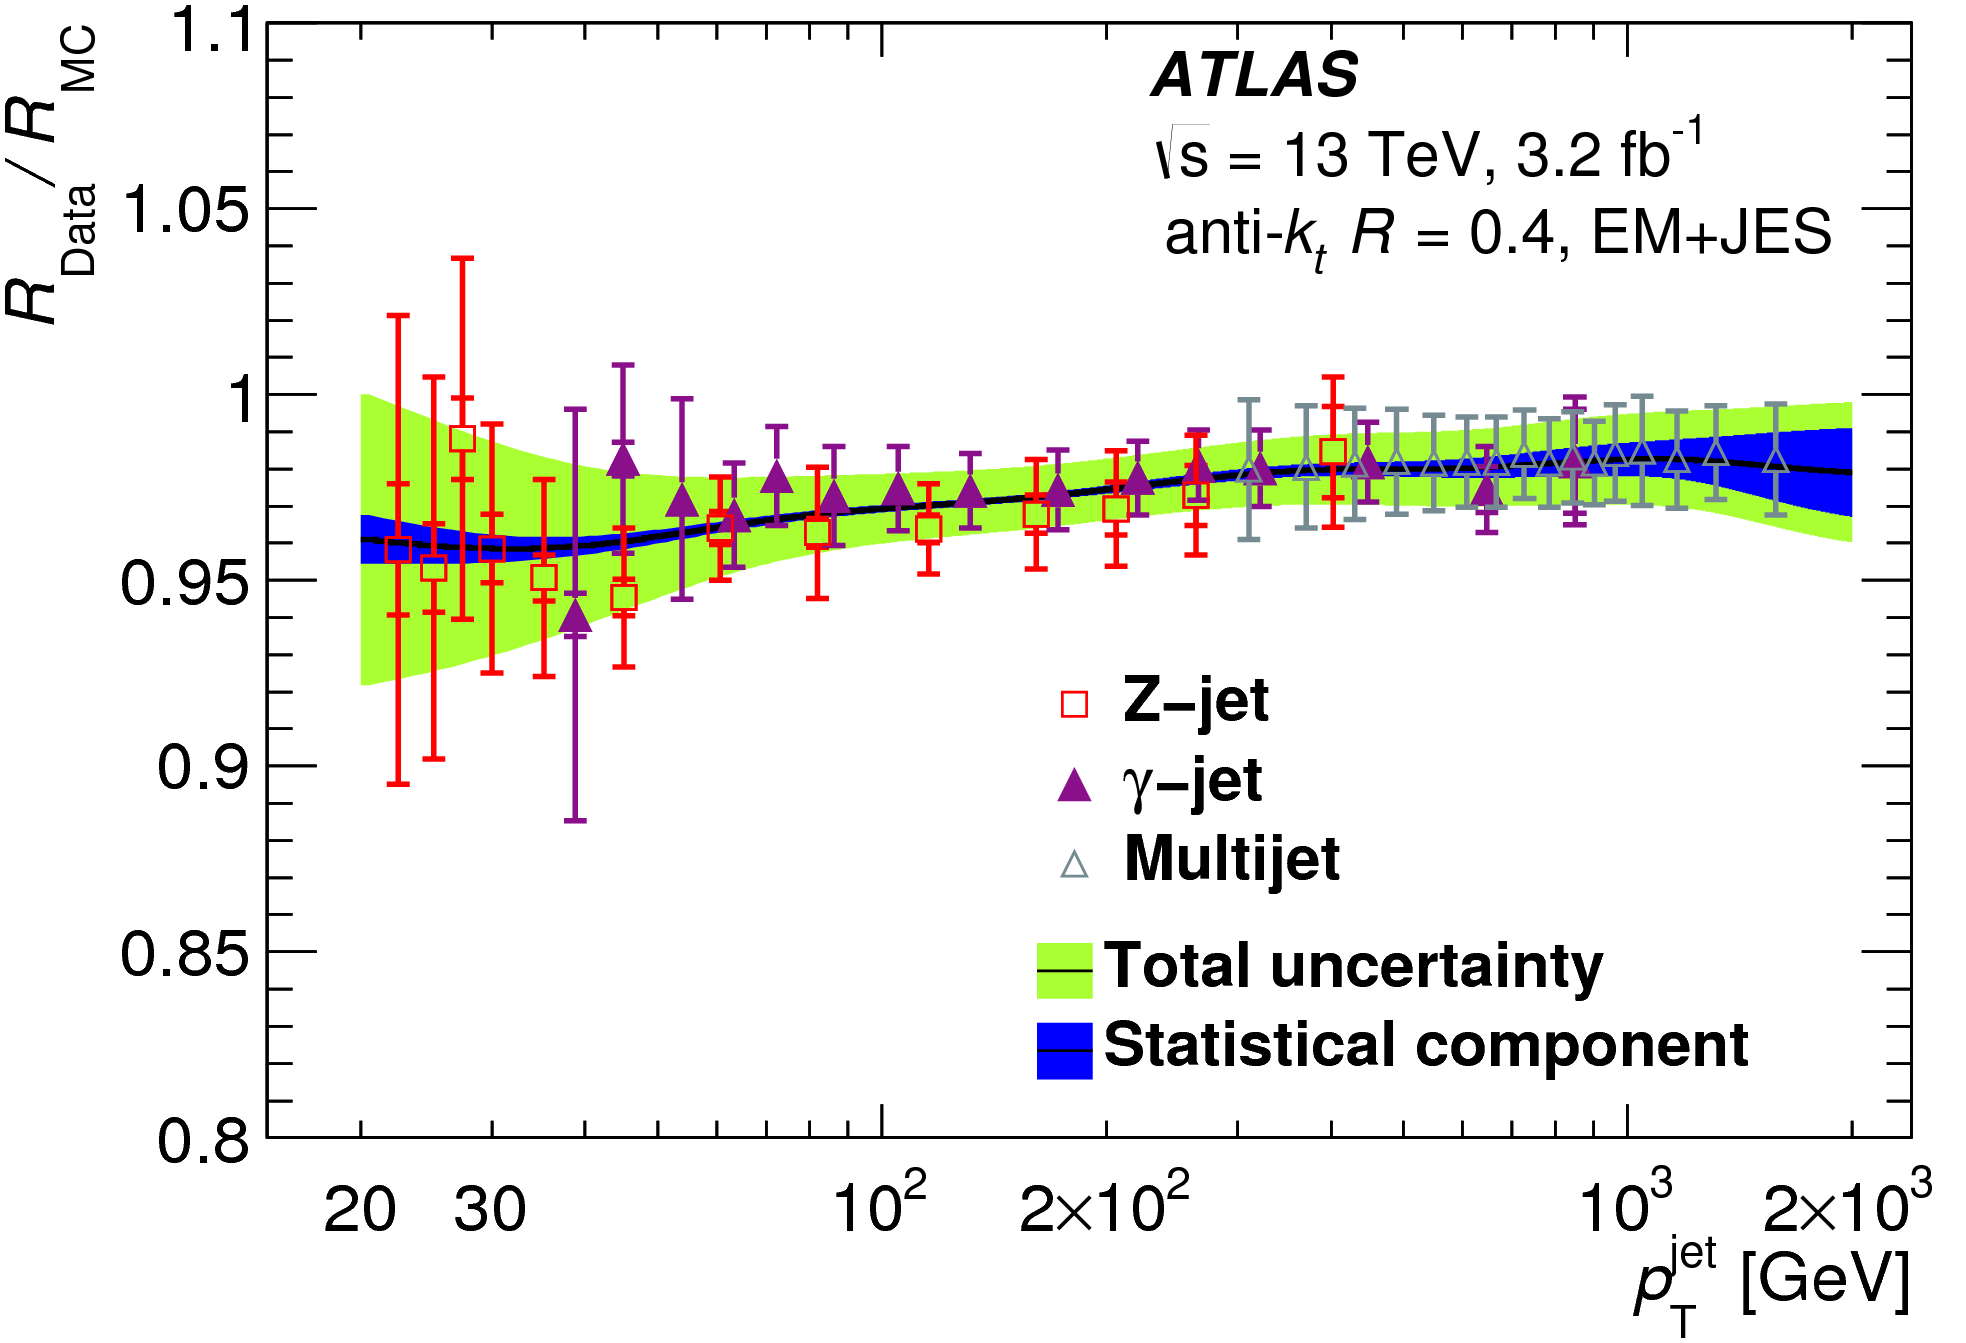
\includegraphics[width=0.7\columnwidth]{figures/SearchStrategy/JES.png}
	\caption{Ratio of the EM+JES jet response in data to that in the nominal MC event generator as a function of jet \pt for $Z$-jet, $\gamma$-jet, and multi-jet in-situ calibrations.  The final derived correction and its statistical and total uncertainty bands are shown.}
	\label{fig:JES}
	
	
\end{figure}

\section{Jet Cleaning}

Jets in events considered by the analysis are subjected to cleaning criteria as defined in Ref.~\cite{JetCleaning} to reject jets which do not originate from a hard scatter, but instead from calorimeter noise, cosmic-ray muons, or beam backgrounds resulting from interactions upstream of the detector.  The variables used in the cleaning selection are:
\begin{itemize}[noitemsep]
	\item $Q^{LAr}_{cell}$, LAr cell quality.  The quadratic difference between the expected and observed pulse shape.
	\item $\langle Q \rangle$, the average jet quality. An energy-weighted average of $Q^{LAr}_{cell}$ for all cells in a jet.
	\item $f^{LAr}_{Q}$, the fraction of LAr calorimeter cells in a jet with poor quality. ($Q^{LAr}_{cell}>4000$)
	\item $f^{HEC}_{Q}$, the fraction of HEC calorimeter cells in a jet with poor quality. ($Q^{LAr}_{cell}>4000$)
	\item $|E_{neg}|$, the sum of all cells in a jet with negative energies.
    \item $f_{EM}$, the fraction of the total jet energy deposited in the EM calorimeter.
    \item $f_{HEC}$, the fraction of the total jet energy deposited in the HEC calorimeter.
    \item $f_{max}$, the maximum energy fraction of any single calorimeter layer.
    \item $f_{ch}$, the ratio of the scalar sum of the $p_T$ of tracks from the primary vertex to the total jet $p_T$.
\end{itemize}
    
A jet is characterized as being bad if it fails any of the following criteria:
\begin{itemize}[noitemsep]
	\item $f_{HEC} > 0.5$ and $|f^{HEC}_{Q}| > 0.5$ and $\langle Q \rangle > 0.8$
	\item $|E_{neg}| >$ 60\,GeV
	\item $f_{EM} > 0.95$ and $f^{LAr}_{Q} > 0.8$ and $\langle Q \rangle > 0.8$ and $|\eta| < 2.8$
	\item $f_{max} > 0.95$ and $|\eta| < 2$
	\item $f_{EM} < 0.05$ and $f_{ch} < 0.05$ and $|\eta| < 2$
	\item $f_{EM} < 0.05$ and $|\eta| \geq 2$
\end{itemize}

The first three selections are used to remove jets caused by noise bursts in the EM or HEC calorimeters, as indicated by a combination of poor cell quality and an overabundance of energy in a given layer.  Calorimeter pulses from noise bursts tend to be very unusual in shape and have large undershoots, and thus large negative energy.  The last three selections target cosmic muons and beam-induced backgrounds, which are usually characterized by large amounts of energy in the hadronic portion of the calorimeter as well as little to no activity in the inner tracker or EM calorimeter.

\section{Mistimed Events in 2015 and 2016 Data}

The Run-1 jet cleaning criteria also included an additional variable $t_{jet}$, the energy-weighted average time of all calorimeter cells in the events.  For Run 2, jet timing is not considered for cleaning.  Jets originating from cosmic muons or beam backgrounds will tend to be out-of-time compared to hard scatter jets, and jets coming from prior or subsequent bunch crossings (BCs) can also be determined.

Early in the 2015 data taking a large deficit was observed in the number of high $p_t$ jets.  This was traced back to a misconfiguration in the Level-1 calorimeter trigger which was causing events with saturated trigger towers to fire the Level-1 Accept one BC too early.  The issue was swiftly addressed, but all data taken prior to this point was unusable for physics (fortunately, only $\sim$80\,pb$^-1$ of data was lost).  Additionally, the problem persisted at a much reduced level for subsequent data taking.  Thankfully, measures were put into place to detect and save mistimed events.

\subsection{The L1Calo Saturated BCID Trigger}

As was discussed in Section~\ref{sec:L1Calo}, to determine which BC an energy deposit is associated to, L1Calo uses two different algorithms which are run on each tower.  The first algorithm is the standard peak finder and is what is used for the vast majority of triggers.  The five readout slices are multiplied against filter coefficients which are determined for each individual tower, but follow the general pattern of having a large multiplier for the central slice and small (or negative) values for the first and last slices.  Between Runs 1 and 2, the system was changed to allow for negative coefficients. The slices are multiplied by their coefficients and then summed together, and this sum is then compared to the sums obtained from windows centered one BC before and after it; if it is found to be a local maximum then it is considered to have peaked in the nominal BC and is added in to the L1 trigger calculations for jets and other objects.  This system is optimized for low energy pulses that are very close to the pedestal value; for larger pulses the peak is much more obvious and this algorithm points to the correct BC for the peak.

In situations where the tower readout saturates things become a bit more complicated; for pulses that saturate only one sample it is trivial to pick out the peak, but in cases where 2+ samples are saturated the peak is less obvious.  A series of studies conducted during Run 1 determined that in these cases the peak always corresponded to the second saturated sample, at least for the energy regime accessible in Run 1.  Thus, the saturated BCID algorithm is always set to point to the sample immediately after the first saturated sample.

The L1Calo system does not have the ability to turn on or off these algorithms based on the pulse in a given event, and so both algorithms independently make a determination on which BC a pulse belongs to.  For small pulses peak finder will point correctly, for pulses with one saturated sample peak finder will point correctly and saturated BCID will point one BC later.  For pulses that saturate many samples, saturated BCID will point to the correct peak while peak finder will point to the same or a later BC.

When a trigger accept is sent by the Central Trigger Processor (CTP), the ATLAS system must then read out the full state of the detector and pass it on to the HLT.  During this time ATLAS enters what is known as Simple Dead Time, a period of approximately 5 BCs where new triggers are not accepted because the system is busy saving the previous event.  As such, any interesting physics events during this period are lost.  So, if Level-1 Accepts are sent during two consecutive BCs, only the first event will be saved and the second will be lost.  For the L1Calo trigger, this meant that even though the two algorithms could point to different BCs, only the event in the first would be saved while the second would be vetoed as it would fall during the simple dead time.

\subsubsection{Identification and Reconstruction of Mistimed Events}

In the case of the early 2015 data, the saturated BCID algorithm was incorrectly configured to point to the first saturated sample rather than the second.  In events where more than one sample was saturated, this meant that the trigger would fire one BC too early and the actual event would fall into the simple dead time and be lost.  Additionally, this error occurred during the 50 ns run configuration of the machine, and so a trigger that was one BC (or 25 ns) early pointed to an empty bunch in the machine.  This meant that the event was not kept in the physics stream but rather placed in a calibration stream looking for noise bursts in the calorimeter.  Additionally, this stream only saved a limited amount of data rather than the full event, so it was not possible to reconstruct the original event.

Once this error was fixed, measures were put into place to guard against future data loss.  A special physics stream was set aside for L1Calo to automatically save all events which were at or near saturation regardless of whether they occurred in empty or filled bunches in the machine.  Additionally, a timing analysis was set up to check all events in this stream for signs of early triggers.  Near the end of 2015 data taking it was discovered that a small number of events were still triggering early, this time due to an unforeseen side effect of the peak finder algorithm.

The typical filter coefficients for the three central readout slices were positive, but the first and last coefficient were negative.  In very highly saturated events where 3 to 4 readout slices were saturated, this first negative coefficient was multiplying a large number in the correct timing window, leading it to give a lower value than a window centered one BC earlier.  This meant that for these very high energy towers the peak finder algorithm would fire one BC early rather than the intended design of firing after the saturated BCID algorithm.  Thankfully, these events were saved by the special L1Calo physics stream, but also tended to be inadvertently saved in the main physics stream as the LHC had switched to 25\,ns.

To identify events which were triggered early by this error, an analysis was set up on the mistimed stream by identifying events with pulses 25\,ns late.  This was done by performing a parabolic fit on all trigger towers above 10 GeV but not at saturation, where the parabola was centered on the largest value of the 5 slices of readout.  The mean value of these L1 tower timings was used to create a timing value for the event, which led to the following selection criteria:

\begin{itemize}[noitemsep]
	\item At least one trigger tower with samples 3-5 saturated, sample 2 below saturation
	\item Event flagged as having been triggered by peak finder algorithm
	\item Event timing $>$ 20\,ns
	\item Tower timing RMS $<$ 3\,ns
	\item At least one tower above 10\,GeV but below saturation in both the EM and hadronic calorimeters.
	\item Vetoing certain lumiblocks with multiple bad events, and events where a large number of EM towers with the same $\phi$ all saturate, indicative of unflagged noise burst events.
\end{itemize}

After all cuts were applied, 110 events were identified as possible early triggers.  These events were then run through the ATLAS reconstruction framework with a special configuration to shift the calorimeter timing to the nominal bunch crossing.  This process corrected the energies of the jets to the proper values, with a few pieces of information missing from the events.  First, a few of the calorimeter channels underestimated their energies due to their readouts saturating.  This is because the gain on the calorimeter channel is chosen based on the value during the nominal bunch crossing, and an early trigger could cause the wrong gain to be chosen.  In studied events, this affected less than 10\% of channels, and the energy was underestimated by $\sim20$\% in such channels, leading to a negligible overall effect.  

Second, the tracking information in the event could not be corrected to the proper BC, and as such the tracks in these corrected events had no correlation to the true event.  Even with this complication nearly all events still passed the primary vertex and charge fraction cleaning criteria, and events that did not were discarded even though they may have been perfectly good.  Finally, muon information was also missing from corrected events, and as such the punch through correction of the global sequential calibration could not be performed correctly.  Testing revealed that this step only affected the energy by a few percent, well below the total JES uncertainties, as shown in Figure~\ref{fig:Mistimed}. After selection, around 90 of these rehabilitated events passed into the final analysis selection, but they comprised some of the highest invariant mass events in the 2015 dataset.

\begin{figure}[ht!]
	\centering
	\subfloat[]{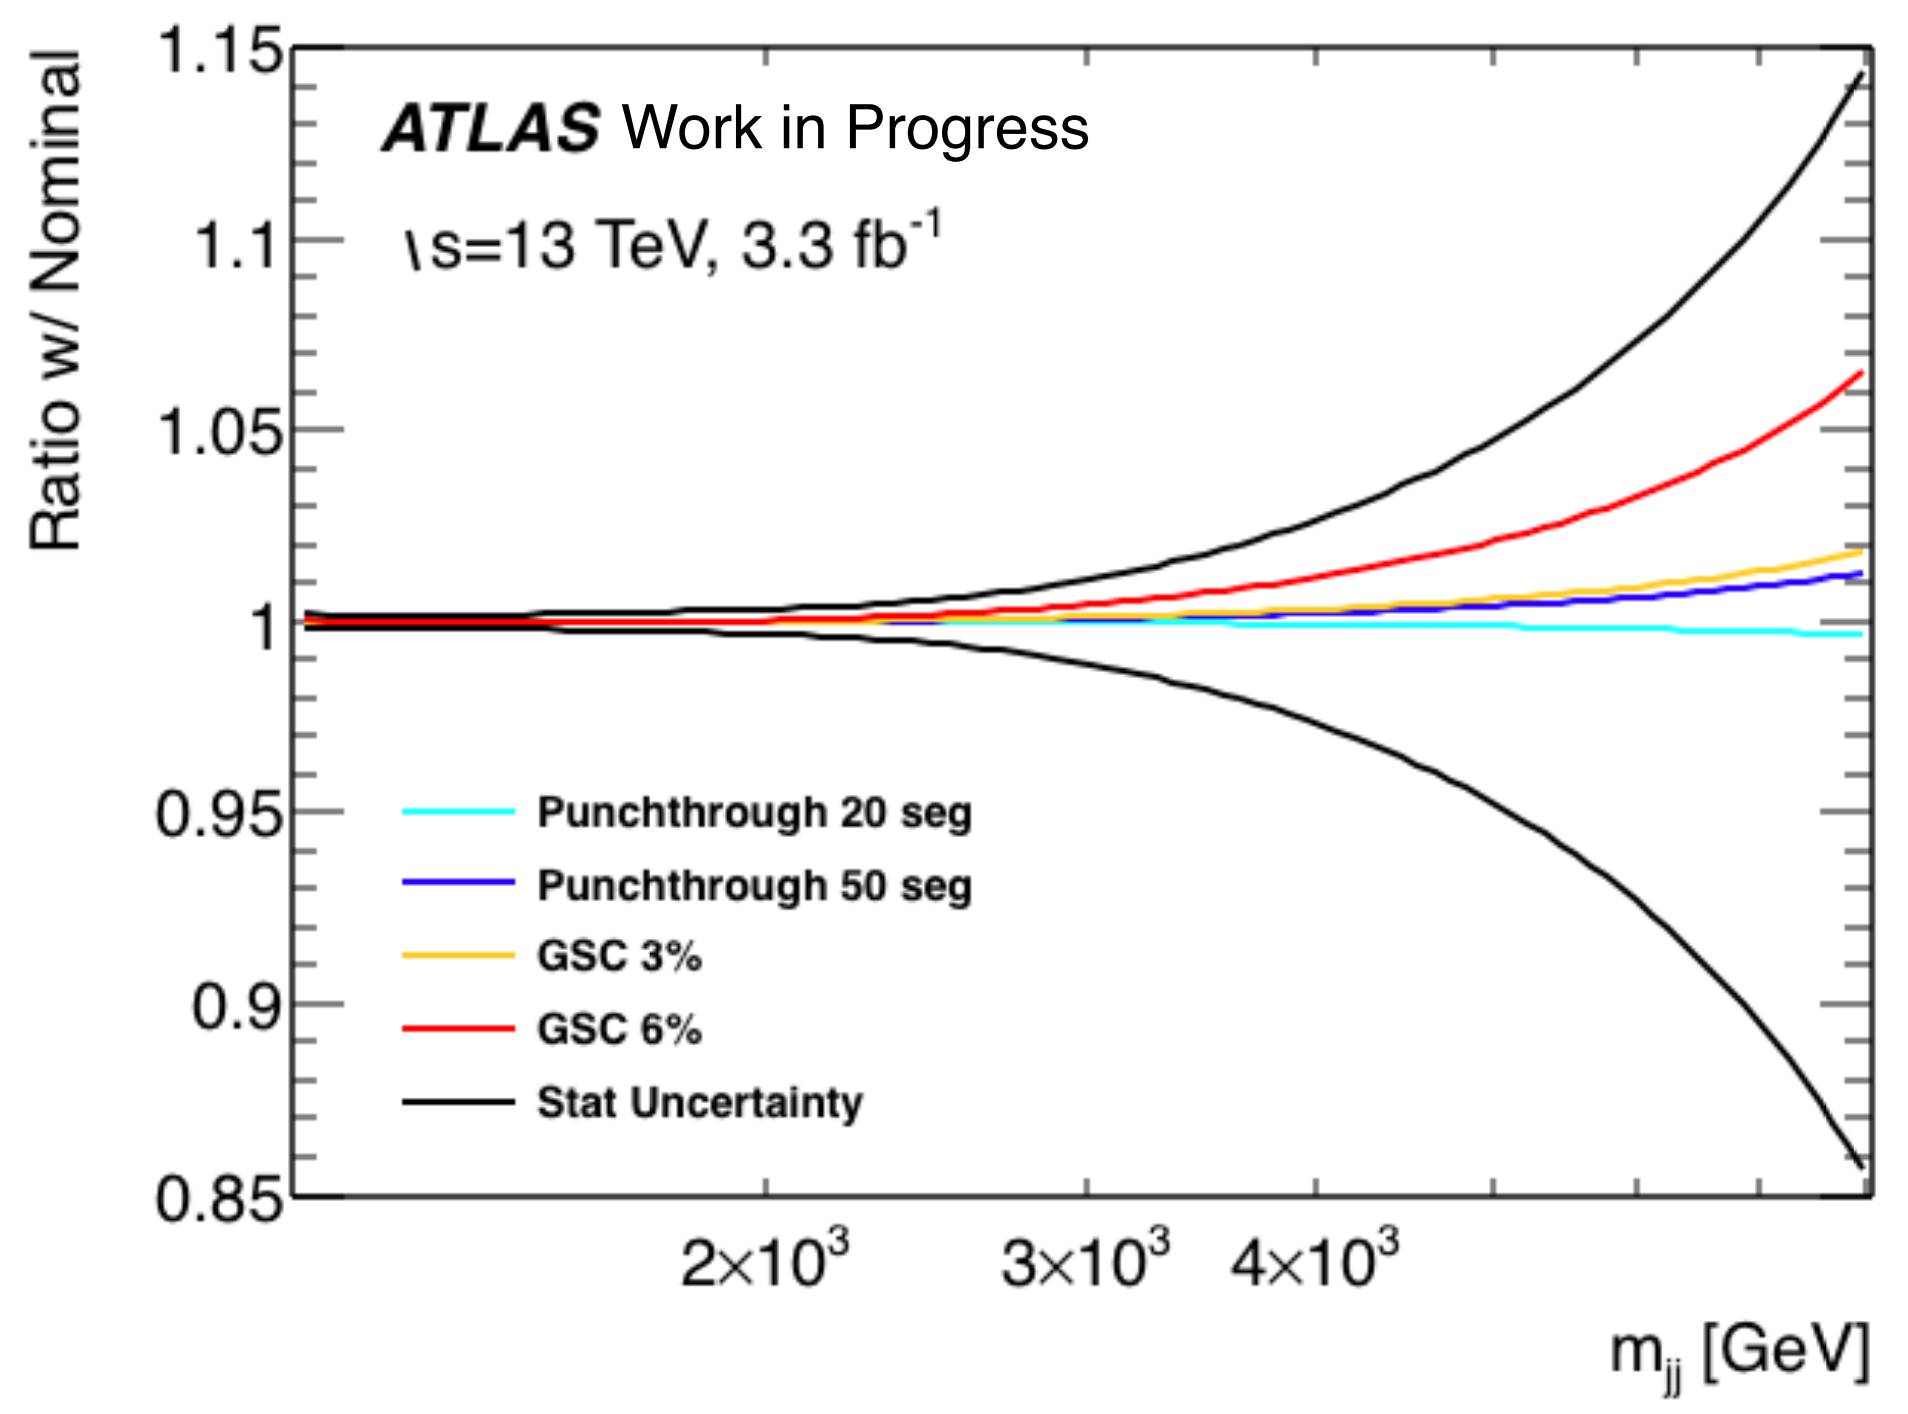
\includegraphics[width=0.46\columnwidth]{figures/SearchStrategy/L1CaloGSC.png}}
	\hspace{0.05\columnwidth}%
	\subfloat[]{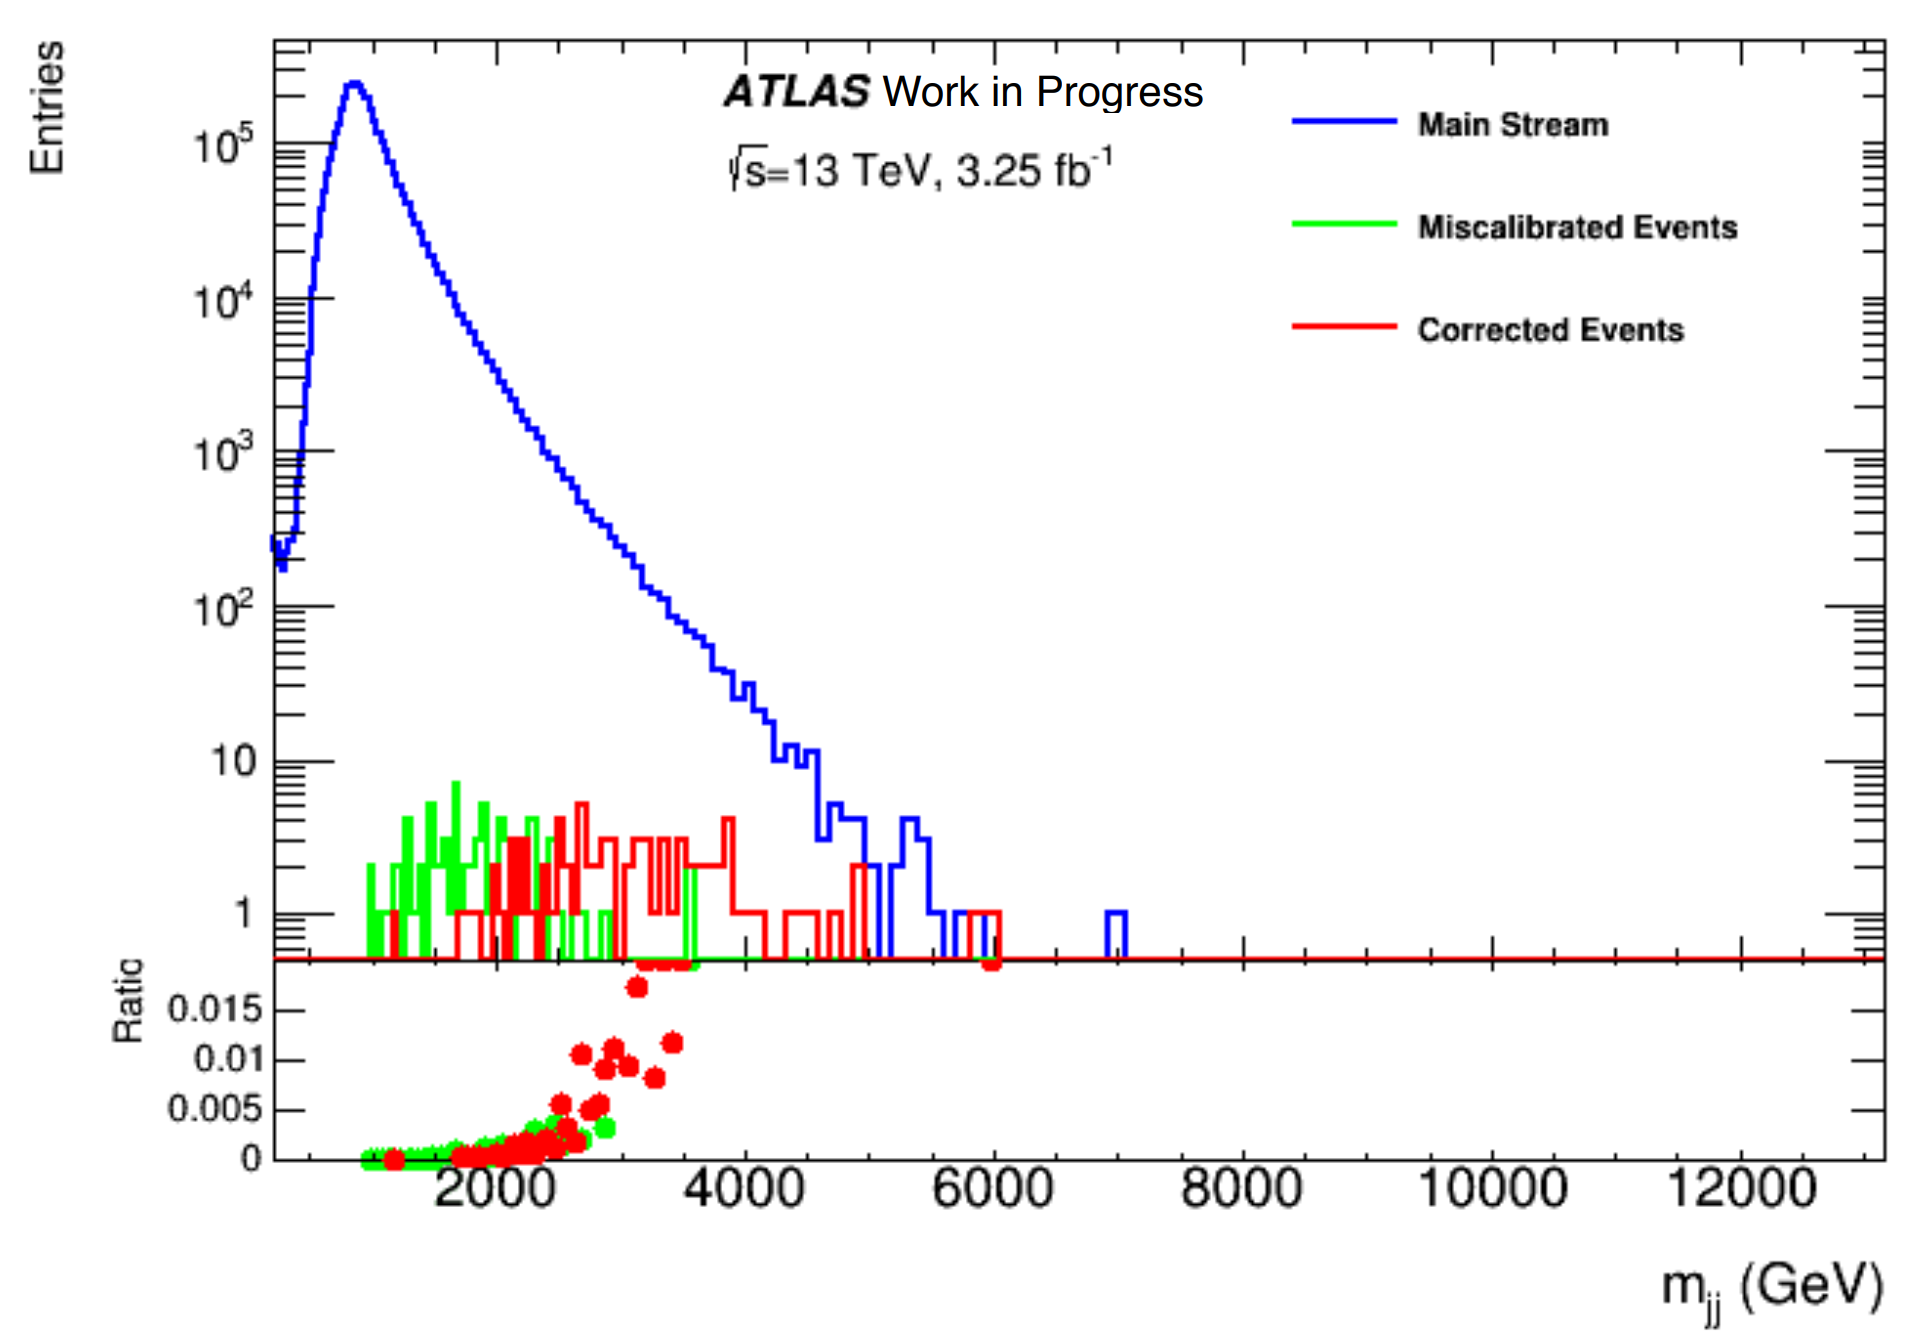
\includegraphics[width=0.48\columnwidth]{figures/SearchStrategy/L1CaloMjj.png}}
	\caption{(a) Comparison of the effect on the \mjj~uncertainty due to missing event information in BCID corrected events compared to the overall statistical uncertainty.  (b) The dijet invariant mass spectrum showing the normal events in blue and the corrected events in red.}
	\label{fig:Mistimed}
\end{figure}

For the 2016 dataset additional measures were put into place to reduce the number of events by forcing peak finder to turn off in towers with four saturated samples; however, a small number still triggered early with three saturated samples.  The cut could not be tightened further without risking late triggers, and as such the few events that snuck through had to be rehabilitated in the same manner.  The early trigger rate for the 2016 dataset was approximately one event/\ifb, and the affected energies were much lower than those in the 2015 events.  The issue of early triggers was fully resolved near the end of 2016 data taking with the introduction of the 80\,MHz sampling algorithm which uses readout with twice the granularity to further refine the BCID identification.